% =====================================================================
%  research_triangle.tex — the three-fields diagram on /Research/
%
%  Source of truth for _assets/research_triangle.svg. Compile with:
%
%      cd figures/tikz
%      ./build.sh
%
%  Colours are NOT final here: each semantic role is drawn in a unique
%  sentinel hex (#FF00xx) that build.sh rewrites into a CSS variable, so
%  the published SVG re-themes with the site's light/dark toggle. Never
%  reuse a sentinel for two different roles.
%
%      figCS   #FF0001  Complex Systems vertex        --fig-cs
%      figIS   #FF0002  Information Sciences vertex   --fig-is
%      figAH   #FF0003  Arts & Humanities vertex      --fig-ah
%      figCore #FF0004  central synthesis label       --fig-core
%      figLine #FF0005  triangle edges                --fig-line
%      figInk  #FF0006  pairwise edge labels          --fig-ink
%      figBg   #FF0007  label backplates (was white)  --fig-bg
% =====================================================================
\documentclass[border=2pt,10pt]{standalone}
\usepackage[T1]{fontenc}
\usepackage{helvet}
\renewcommand{\familydefault}{\sfdefault}
\usepackage{tikz}
\usetikzlibrary{calc}

\definecolor{figCS}{HTML}{FF0001}
\definecolor{figIS}{HTML}{FF0002}
\definecolor{figAH}{HTML}{FF0003}
\definecolor{figCore}{HTML}{FF0004}
\definecolor{figLine}{HTML}{FF0005}
\definecolor{figInk}{HTML}{FF0006}
\definecolor{figBg}{HTML}{FF0007}

\begin{document}
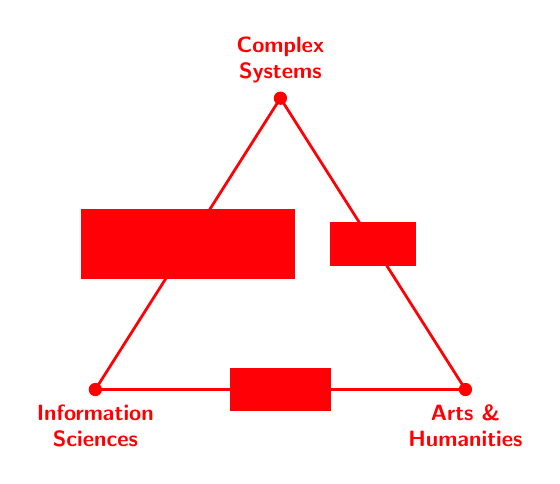
\begin{tikzpicture}
    % vertices
    \coordinate (CS) at (0,2.2);
    \coordinate (IS) at (-2.35,-1.5);
    \coordinate (AH) at (2.35,-1.5);
    % triangle edges
    \draw[figLine,line width=1pt] (CS)--(IS)--(AH)--cycle;
    % vertex dots
    \fill[figCS] (CS) circle (2.4pt);
    \fill[figIS] (IS) circle (2.4pt);
    \fill[figAH] (AH) circle (2.4pt);
    % field names at the corners
    \node[text=figCS,font=\footnotesize\bfseries,align=center,above=2pt] at (CS) {Complex\\Systems};
    \node[text=figIS,font=\footnotesize\bfseries,align=center,below=2pt] at (IS) {Information\\Sciences};
    \node[text=figAH,font=\footnotesize\bfseries,align=center,below=2pt] at (AH) {Arts \&\\Humanities};
    % pairwise terms, on the edge between each pair of fields (backplate breaks the line)
    \node[fill=figBg,inner sep=1.5pt,text=figInk,font=\scriptsize,align=center] at ($(CS)!0.5!(IS)$) {semi-automated\\cataloging + knowledge\\ discovery};
    \node[fill=figBg,inner sep=1.5pt,text=figInk,font=\scriptsize,align=center] at ($(CS)!0.5!(AH)$) {cultural\\evolution};
    \node[fill=figBg,inner sep=1.5pt,text=figInk,font=\scriptsize,align=center] at ($(IS)!0.5!(AH)$) {digital\\humanities};
    % center: the synthesis of all three (label intentionally omitted)
\end{tikzpicture}
\end{document}
